\newpage
\section{Prototype Pattern}

Prototype pattern refers to creating duplicate object while keeping performance in mind. This type of design provides one of the best ways to create an object.
This pattern involves implementing a prototype interface which tells to create a clone of the current object. This pattern is used when creation of object directly is costly. For example, an object is to be created after a costly database operation. We can cache the object, returns its clone on next request and update the database as and when needed thus reducing database calls.
\subsection{Class Diagram}

\begin{figure}[h]
\centering
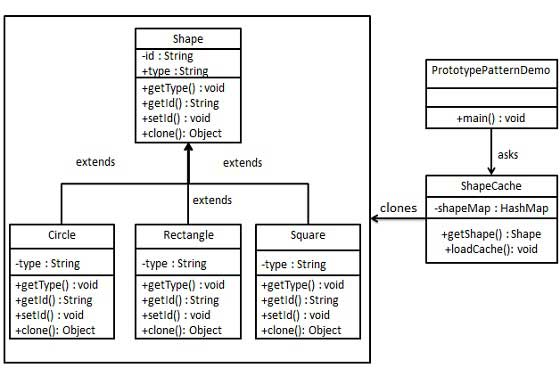
\includegraphics[scale=0.7]{prototype}
\caption{Class Diagram of Prototype Pattern}
\end{figure}

\newpage
\subsection{Source Code (Java)}

\subsubsection{Shape Class}

\begin{minted}{java}
public abstract class Shape implements Cloneable {
   
   private String id;
   protected String type;
   
   abstract void draw();
   
   public String getType(){
      return type;
   }
   
   public String getId() {
      return id;
   }
   
   public void setId(String id) {
      this.id = id;
   }
   
   public Object clone() {
      Object clone = null;
      
      try {
         clone = super.clone();
         
      } catch (CloneNotSupportedException e) {
         e.printStackTrace();
      }
      
      return clone;
   }
}
\end{minted}

\subsubsection{Rectangle Class}

\begin{minted}{java}
public class Rectangle extends Shape {

   public Rectangle(){
     type = "Rectangle";
   }

   @Override
   public void draw() {
      System.out.println("Inside Rectangle::draw() method.");
   }
}
\end{minted}

\subsubsection{Square Class}

\begin{minted}{java}
public class Square extends Shape {

   public Square(){
     type = "Square";
   }

   @Override
   public void draw() {
      System.out.println("Inside Square::draw() method.");
   }
}
\end{minted}

\subsubsection{Circle Class}

\begin{minted}{java}
public class Circle extends Shape {

   public Circle(){
     type = "Circle";
   }

   @Override
   public void draw() {
      System.out.println("Inside Circle::draw() method.");
   }
}
\end{minted}

\subsubsection{ShapeCache Class}

\begin{minted}{java}
import java.util.Hashtable;

public class ShapeCache {
	
   private static Hashtable<String, Shape> shapeMap  = new Hashtable<String, Shape>();

   public static Shape getShape(String shapeId) {
      Shape cachedShape = shapeMap.get(shapeId);
      return (Shape) cachedShape.clone();
   }

   // for each shape run database query and create shape
   // shapeMap.put(shapeKey, shape);
   // for example, we are adding three shapes
   
   public static void loadCache() {
      Circle circle = new Circle();
      circle.setId("1");
      shapeMap.put(circle.getId(),circle);

      Square square = new Square();
      square.setId("2");
      shapeMap.put(square.getId(),square);

      Rectangle rectangle = new Rectangle();
      rectangle.setId("3");
      shapeMap.put(rectangle.getId(), rectangle);
   }
}
\end{minted}

\subsubsection{Driver Class}

\begin{minted}{java}
public class PrototypePatternDemo {
   public static void main(String[] args) {
      ShapeCache.loadCache();

      Shape clonedShape = (Shape) ShapeCache.getShape("1");
      System.out.println("Shape : " + clonedShape.getType());		

      Shape clonedShape2 = (Shape) ShapeCache.getShape("2");
      System.out.println("Shape : " + clonedShape2.getType());		

      Shape clonedShape3 = (Shape) ShapeCache.getShape("3");
      System.out.println("Shape : " + clonedShape3.getType());		
   }
}
\end{minted}

\subsection{Output}

\begin{minted}{java}
Shape : Circle
Shape : Square
Shape : Rectangle
\end{minted}